\begin{figure}[h]
    \centering
    \vspace{1em}
    \tikzset{every picture/.style={line width=0.75pt}} %set default line width to 0.75pt        
    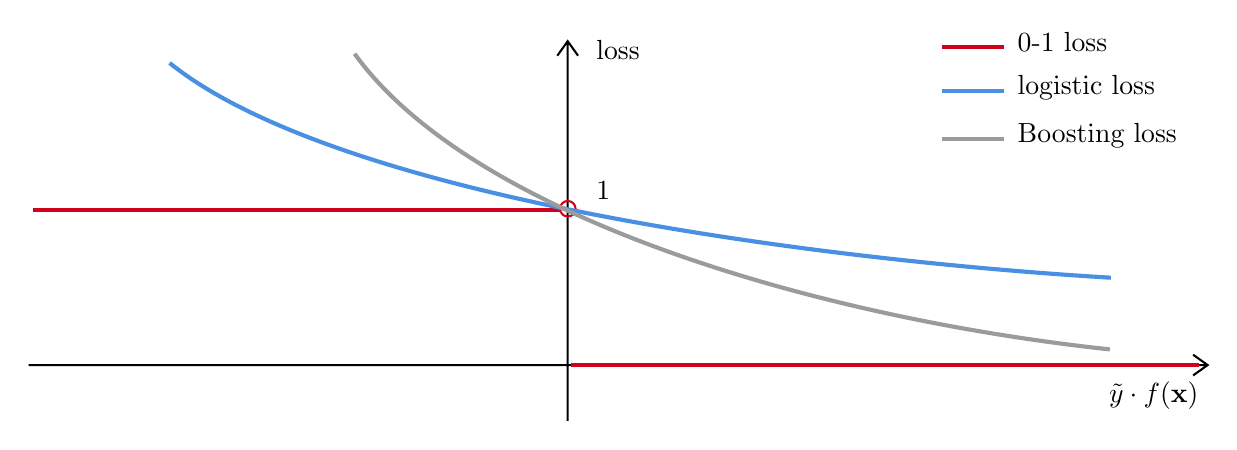
\begin{tikzpicture}[x=0.75pt,y=0.75pt,yscale=-1,xscale=1]
    %uncomment if require: \path (0,303); %set diagram left start at 0, and has height of 303

    %Shape: Axis 2D [id:dp3583783281791968] 
    \draw [color={rgb, 255:red, 0; green, 0; blue, 0 }  ,draw opacity=1 ][line width=0.75]  (50,230.06) -- (618,230.06)(309.68,74) -- (309.68,257) (611,225.06) -- (618,230.06) -- (611,235.06) (304.68,81) -- (309.68,74) -- (314.68,81)  ;
    %Straight Lines [id:da9462308845100503] 
    \draw [color={rgb, 255:red, 208; green, 2; blue, 27 }  ,draw opacity=1 ][line width=1.5]    (311.05,230.06) -- (613.89,230.06) ;
    %Shape: Circle [id:dp030187270009231715] 
    \draw  [color={rgb, 255:red, 208; green, 2; blue, 27 }  ,draw opacity=1 ] (306,154.74) .. controls (306,152.67) and (307.67,151) .. (309.74,151) .. controls (311.8,151) and (313.48,152.67) .. (313.48,154.74) .. controls (313.48,156.8) and (311.8,158.48) .. (309.74,158.48) .. controls (307.67,158.48) and (306,156.8) .. (306,154.74) -- cycle ;
    %Straight Lines [id:da8641638161872071] 
    \draw [color={rgb, 255:red, 208; green, 2; blue, 27 }  ,draw opacity=1 ][line width=1.5]    (51.89,155.28) -- (306,155.28) ;
    %Curve Lines [id:da8231370476695449] 
    \draw [color={rgb, 255:red, 74; green, 144; blue, 226 }  ,draw opacity=1 ][line width=1.5]    (117.89,84.51) .. controls (199.89,150.51) and (436.37,179.96) .. (571.37,187.96) ;
    %Curve Lines [id:da2244247175359496] 
    \draw [color={rgb, 255:red, 155; green, 155; blue, 155 }  ,draw opacity=1 ][line width=1.5]    (207,80.06) .. controls (264,159.06) and (430.89,207.51) .. (570.89,222.51) ;
    %Straight Lines [id:da0642709600211735] 
    \draw [color={rgb, 255:red, 208; green, 2; blue, 27 }  ,draw opacity=1 ][fill={rgb, 255:red, 208; green, 2; blue, 27 }  ,fill opacity=1 ][line width=1.5]    (490,77) -- (520,77) ;
    %Straight Lines [id:da7140393011733781] 
    \draw [color={rgb, 255:red, 74; green, 144; blue, 226 }  ,draw opacity=1 ][line width=1.5]    (490,98) -- (520,98) ;
    %Straight Lines [id:da32663581505367] 
    \draw [color={rgb, 255:red, 155; green, 155; blue, 155 }  ,draw opacity=1 ][line width=1.5]    (490,121) -- (520,121) ;

    % Text Node
    \draw (525,68) node [anchor=north west][inner sep=0.75pt]   [align=left] {0-1 loss};
    % Text Node
    \draw (525,89) node [anchor=north west][inner sep=0.75pt]   [align=left] {logistic loss};
    % Text Node
    \draw (525,112) node [anchor=north west][inner sep=0.75pt]   [align=left] {Boosting loss};
    % Text Node
    \draw (322,140.4) node [anchor=north west][inner sep=0.75pt]    {$1$};
    % Text Node
    \draw (322,72) node [anchor=north west][inner sep=0.75pt]   [align=left] {loss};
    % Text Node
    \draw (569,236.4) node [anchor=north west][inner sep=0.75pt]    {$\tilde{y} \cdot f(\mathbf{x})$};

    \end{tikzpicture}

    \caption{Example figure}
    \label{fig-eg}
\end{figure}